\documentclass[acmtog, anonymous=false,review=false, nonacm, balance = false]{acmart}
%%
%% \BibTeX command to typeset BibTeX logo in the docs
\AtBeginDocument{%
  \providecommand\BibTeX{{%
    \normalfont B\kern-0.5em{\scshape i\kern-0.25em b}\kern-0.8em\TeX}}}

\usepackage{xcolor}
\usepackage{colortbl}
\usepackage[ruled,vlined]{algorithm2e}

\newcommand{\reffig}[1] {Fig.~\ref{fig:#1}}
\newcommand{\refalg}[1] {Alg.~\ref{alg:#1}}

\newcommand{\dave}[1]{{\bf\textcolor[rgb]{0.2,0.2,0.8}{Dave: #1}}}

%%% Math Symbols below %%%%
\newcommand{\real}{{\rm I\!R}}
\newcommand{\vc}[1]{\mathbf{#1}}
\newcommand{\refX}{\mathbf{X}}
\newcommand{\defX}{\mathbf{x}}
\newcommand{\Jnurbs}{J}
\newcommand{\ident}{I}
\newcommand{\Pmat}{P}
\newcommand{\Pco}{\vc{c}}
\newcommand{\tr}{\vc{t}}
\newcommand{\Pmatx}  {\begin{pmatrix}\Pmat\left(\refX\right) & \ident \end{pmatrix}}
\newcommand{\Pmatxuv} {\begin{pmatrix}\Pmat\left(\refX\left(u,v)\right)\right) & \ident \end{pmatrix}}
\newcommand{\Pcox} {\begin{pmatrix} \Pco\\ \tr \end{pmatrix}}

\acmSubmissionID{230}
\newcommand\myworries[1]{\textcolor{red}{#1}}

%%%%%%%%%%%%%%%%%%%%%%%%%%%%%%%%%%%%%%%%
% Inverting Colors to save my eye balls
%\usepackage{xcolor}
%\pagecolor[rgb]{0.1,0.12,0.15}
%\color[rgb]{.9,.9,.95}
%%%%%%%%%%%%%%%%%%%%%%%%%%%%%%%%%%%%%%%%

\citestyle{acmauthoryear}

\begin{document}

\title{The Shape Matching Element Method: Direct Animation of Curved Surface Models}

\author{Ty Trusty}
\affiliation{%
 \institution{University of Toronto}
 \streetaddress{40 St. George Street}
 \city{Toronto}
 \state{ON}
 \country{Canada}
 \postcode{M5S 2E4}
}
\email{trusty@cs.toronto.edu}
%
\author{Honglin Chen}
\affiliation{%
  \institution{University of Toronto}
  \streetaddress{40 St. George Street}
  \city{Toronto}
  \state{ON}
  \country{Canada}
  \postcode{M5S 2E4}
}
\email{chl9797@cs.toronto.edu}
%
%
\author{David I.W. Levin}
\affiliation{%
 \institution{University of Toronto}
 \streetaddress{40 St. George Street}
 \city{Toronto}
 \state{ON}
 \country{Canada}
 \postcode{M5S 2E4}
}
\email{diwlevin@cs.toronto.edu}



%% A "teaser" image appears between the author and affiliation
%% information and the body of the document, and typically spans the
%% page.
\begin{teaserfigure}
  \includegraphics[width=\textwidth]{figures/teaser_castle.pdf}
  \caption{Using the shape matching element method we can directly simulate this NURBS surface model of a bouncy castle as a volumetric elastic object without the need for volumetric meshing of any kind.}
  \label{fig:teaser}
\end{teaserfigure}

\begin{abstract}
We introduce a new method for direct physics-based animation of volumetric curved models, represented using NURBS surfaces.  
Our technical contribution is the Shape Matching Element Method (SEM).
SEM is a completely meshless algorithm, the first to simultaneously 
be robust to gaps and overlaps in geometry, 
be compatible with standard constitutive models and time integration schemes, support contact and frictional interactions  
and to preserve feature correspondence during simulation which enables editable simulated output. 
We demonstrate the efficacy of our algorithm by producing compelling physics-based animations from a variety of curved input models.
\end{abstract}

\maketitle

\section{Introduction}

The consumption of geometric surface models by physics-based animation algorithms is fraught with difficulty. 
For volumetric objects, this process often involves identifying and discretizing the interior of the modelled object, 
typically either as a tetrahedral or hexahedral mesh.%
This procedure is both expensive and difficult, especially if the surface model is constructed from higher-order boundary
representations, or if the volumetric discretization is required to be conforming or feature aligned. 
Removing explicit volumetric discretization from the physics-based-animation pipeline can avoid these difficulties and 
also provide a more unified modelling and simulation experience. 

NURBS (Non-uniform Rational B Splines) are a popular higher-order modelling primitive which 
are used for computer-aided design (CAD), computational fabrication and computer animation. 
NURBS primitives were the first geometric representation used for physics-based animation~\cite{10.1145/37402.37427}, yet,
despite over three decades of research, animation of curved models such as those built with NURBS, remains a challenge.

Isogeometric Analysis (IGA) is a physics simulation methodology that uses the control variables of the NURBS model
as the degrees-of-freedom (DOFS) of the simulation itself. 
Unfortunately IGA approaches for volumetric objects still require background volumetric structures, typically
regular grids that make satisfaction of boundary conditions difficult (which makes collision resolution hard)
or more complicated cut-cell grids which introduce non-trivial root finding problems into the mix. 
Crucially, these simulation schemes typically assume models arise from engineering applications and meet tight geometric
criteria such as that the mesh is manufacturable. 
These inputs are much cleaner than those produced by a typical animation modeller. 

% In this paper we present a new finite element method for isogeometric, physics-based animation of NURBs models.
% Crucially our method is boundary only, and requires no volumetric meshes (thus avoiding their inherent complications), grids or cutcells of any kind
% Our method does not need an explicit labelling of the inside/outide of the simulated model
% Does not require nurbs patches in an object to be explicitly joined
% Input is just the raw NURBs model with no additional information or annotations
% The resulting simulation algorithm is compatiable with nonlinear continuum mechanics material models as well as 
% standard methods for contact resolution. 

We present the first truly meshless (no volumetric discretization generated) algorithm for direct, nonlinear elastodynamic simulation of NURBs models. 
Our nonlinear elastodynamic simulation scheme requires only a boundary description of the object (we do not strictly require a solid model) and
approriate physical parameters.  
Because we explicitly use the NURBS boundary representation in the simulation, it is straightforward to handle
Dirichlet and Neumann boundary conditions and to apply contact resolution. 
Crucially because we broadly target animation not necessarily simulation for engineering or manufacturing, we don't require that models
satisfy the rigourous geometric requirements common for these applications

Our approach draws inspiration from the recently developed Virtual Element Method (VEM) for solving partial differential equations on domains tiled with arbitrary polygons.
We establish a connection between VEM and the well-known shape matching simulation algorithm. This allows us 
to derive equations of motion for an arbitrary curved surface model, made of NURBS, via Lagrangian Mechanics. 
Importantly, we show how to replace volumetric data structures for integration and blending weight computation with ray casting approaches which enables
our meshless approach to elastodynamic physically-based animation.

% Modelling -> Animation -> Rendering
% Use physics for animation which requires conversion from modelling to simulation representation
% for volumetric objects this conversion invovles identififyin and meshing the interior of the modelled object and that's hard
% especially difficult if object surface is described by higher-order boundary representations. 
% Ideally we would have a more direct method of translating our surface model into a volumetric, simulatable form
%
% NURBs  are an oft-used higher order modelling primitive popular for CAD and Computer Graphics for which nice modelling tools exist
% Rhinocerous 3D and Fusion 360.
% Despite lots of work performing physics-based animation on NURBS models is hard
% robustly uilding a volumetric polygonal mesh that simulataneously maintains a corresonpondence to the model surface is an open-research problem
% Isogeometric approaches which directly use the NURBs primitives as simulation variables require additional background grids, complex cutcell algorithms
% and often must rely on soft boundary conditions.
%
% Want to say there is an advantage to avoiding constructing volumetric representations because it costs time and adds complexity
% that;s our goal to provide an alternative, the first truly meshless approach to IGA which maintains a tightt mapping to the boundary
% In this paper we present a new finite element method for isogeometric, physics-based animation of NURBs models.
% Crucially our method is boundary only, and requires no volumetric meshes (thus avoiding their inherent complications), grids or cutcells of any kind
% Our method does not need an explicit labelling of the inside/outide of the simulated model
% Does not require nurbs patches in an object to be explicitly joined
% Input is just the raw NURBs model with no additional information or annotations
% The resulting simulation algorithm is compatiable with nonlinear continuum mechanics material models as well as 
% standard methods for contact resolution. 
%
% crucially because we broadly target animation not necessarily simulation for engineering or manufacturing we don't require that models
% satisfy rigourous geometric requirements common for these applications
%
% Our approach relies on the recently developed Virtual Element Method for solving PDEs on domains tiled with arbitrary polygons.
% By establsihing the connection between VEM and the well-known shape matching simulation algorithm we derive equations of motion sfor 
% an arbitrary NURBS model using Lagrangian Mechanics. We avoid using volumetric data structures for integration by demonstrating that 
% raycasting provides a fast and reliable alternative. In combination, our contributions amount to the first algorithm for 
% isogeometric elastodynamics of volumetric structures that is truly meshless (introducing no auxilillary volumetric data structures) 
% which serves to close the considerable gap betweeen modelling and physics-based animation. 
%
% Desiderata for a sucessful algorithm for PBA 
% No volumetric mesh creation
% Support for Nonlinear Constitutive Models
% Support for standard Collision 
% DOFS on the Boundary (useful for boundary conditions, contact)
% Automatic determination of model volume
% Non-manufacturable models 
% Code Available 

%limitations
% sometimes you want some volumetric dofs to better resolve internal behaviour
\section{Related Work}

%% Set the scene
Geometric modeling is a necessary precursor to physics-based animation, however differing geometric representations for modelling and simulation often require
time-consuming, complex geometry processing pipelines. 
For instance, the popular tetrahedral finite element approach for simulating solid elastodynamics requires robust algorithms for converting input surface geometry into 
a volumetric tetrahedral mesh. This is a difficult problem and while significant progress has been~\cite{10.1145/2343483.2343501} made,
even the most robust volumetric methods~\cite{Hu:2018:TMW:3197517.3201353} can be time consuming, fail to maintain correspondence between the input model and output simulation mesh,
and don't work directly on curved surface representations such as NURBS.  

%% Outline desiderata for success
%- no meshing of any kind, no tet, hex cut cells, nothing
%- simulation can be directly imported and edited in modelling software
%- supports standard continuum mechanics constitutive models
%- supports different time integrators (can show a few maybe linearly implicit, fully implicit and RK4 ?)

For many physically-based animation tasks, it would be desirable to bypass volumetric meshing entirely and directly simulate the geometric model.
An ideal approach would avoid meshing of any kind (no volumetric meshes or cutcells), support continuum mechanics type constitutive models 
and energies that have become standard in physics-based animation pipelines, be compatible with a wide range of time integration schemes and
ensure that simulation output can be edited in the same modelling software used to create the input (important for post-processing). 
Finally, our method should put only moderate constraints on input model quality to facilitate ease-of-use.

\emph{Isogeometric Analysis}~\cite{10.1002/9780470749081.ch7} endeavors to perform simulation directly on the NURBS output from 
Computer-Aided Design (CAD) software. Initial attempts used NURBS surfaces to represent the mid-surface of thin objects~\cite{10.1145/176579.176580}.
Initial attempts at volumetric simulation relied on volumetric NURBS~\cite{10.1007/978-3-642-03596-8_2} but were limited to a narrow class of geometries.
Finite volume methods are applicable to more general geometries~\cite{HEINRICH20121645,10.1002/nme.2311} but require a volumetric mesh be generated.
Modern approaches are constructed around the extended finite element method which enriches the standard finite element basis with discontinuous basis functions
to enable improved boundary handling~\cite{https://doi.org/10.1002/nme.3120,10.1007/s00466-013-0854-7,https://doi.org/10.1002/nme.4852,SAFDARI2016373,10.1145/3355089.3356576}. 
These methods typically start with an easy-to-generate structured volumetric mesh (tetrahedral or hexahedral), ``cutting'' the NURBS geomtric model against
it to enable boundary handling (such a mesh is called a \emph{cutcell} mesh). 
Like volumetric meshing, this cutting operation can be difficult and our ideal method would avoid it if possible. 
Some cutcell algorithms assume engineering/manufacturing quality input, which puts tight requirements on input models quality~\cite{10.1145/3355089.3356576}.
Finally these approaches require additional mechanisms to ensure that simulation results lie inside the shape space of the input model's primitives,
increasing complexity. 

\emph{Shape Matching} is a meshless approach to physics-based animation~\cite{10.1145/1073204.1073216,10.1145/2019406.2019438} and geometry processing~\cite{10.1111/j.1467-8659.2012.03171.x}
built around shape registration. The algorithm has been extended from volumetric triangle mesh input to cloth~\cite{10.2312/PE/vriphys/vriphys08/039-046} to particles~\cite{10.1145/1964921.1964987}
and even to visual geometry for video games~\cite{10.1145/2994258.2994260}. 
Shape Matching is fast~\cite{10.1145/1275808.1276480,10.5555/1632592.1632606} and meshless, but state-of-the-art methods require 
additional modeling input to position simulation primitives ~\cite{0.1145/1964921.1964987} or limit simulation primitives to be 
collections of convex polytopes~\cite{10.1145/2994258.2994260}.
Finally, Shape Matching is tightly coupled to the position-based dynamics~\cite{muller2007position}
time integration methodology. 
While incredibly performant, this approach is incompatible with the constitutive models that are popular for physics-based animation as well as 
other time integration schemes. 
The popular Projective Dynamics algorithm~\cite{10.1145/2601097.2601116} enables a more flexible Shape Matching implementation but is still limited to a subset of
constitutive models for elastic solids. 

To alleviate these restrictions we can to turn to other meshless methods popular in computer graphics and 
engineering~\cite{10.1145/1028523.1028542,https://doi.org/10.1002/fld.1650200824,10.1145/1778765.1778776,10.1145/2010324.1964968, 10.1145/1944846.1944855}.
These support more advanced constitutive models and integration schemes but often require background integration meshes and lose the direct connection with
modelling geometry. 
Like cutcell-based, Isogeometric Analysis approaches, additional constraints must be added to ensure that simulation output can be represented by the input model.
Given this, we conclude that there is no existing algorithm that meets our desiderata for success. 

Our algorithm takes the Shape Matching approach as inspiration, but rather than follow the PBD formalism, we interpret Shape Matching as a 
Virtual Element Method (VEM)~\cite{10.1142/S0218202512500492,10.1142/S021820251440003X}. Virtual Elements are an extension of 
mimetic finite differences~\cite{10.1142/S0218202505000832,10.1016/j.jcp.2013.07.031} to weak-form variational problems. 
VEM relaxed the mesh generation requirements of finite element method by enabling the solution of partial differential equations
on domains partitioned with arbitrary polytopes~\cite{10.1145/3386569.3392389}. 
The solution inside each polytope is approximated using a polynomial function of a specified order.
VEM typically assumes that the boundary of the the problem domain is described by a piecewise linear complex
which makes its standard formulation incompatible with our NURBS based input geometry. 


\subsection*{Contributions} 
In this paper we develop a new Shape Matching-based, Virtual Element Method which is directly compatible 
with NURBS input geometry rather than piecewise linear surfaces. 
Furthermore, we improve the expressivity of the VEM basis by using a shape blending approach inspired by
algorithms for skinning~\cite{skinningcourse:2014}.
Our method is entirely meshless (requiring no volumetric meshes or cutcells) and is compatible with standard constitutive models and time integrators.
It guarantees that simulation output is directly consumable by the input modeling software and can ingest models which include large gaps,
intersections and disconnected primitives without additional user input. 
These features mean that our algorithm is the first truly meshless approach for the simulation of NURBS models for physics-based animation.


%\subsection{Virtual Element and other Element Methods}
%\begin{enumerate}
    %\item \textit{Mimetic Finite Differences} \cite{10.1142/S0218202505000832} \cite{10.1016/j.jcp.2013.07.031} (they double dipped!): Considered a close relative to VEM and framed as the predecessor to VEM (in VEM papers). I still haven't read on MFD yet. From PolyDDF: "extension of finite volume and finite difference techniques to polygons that first discretizes a prime operator (typically, the gradient or the divergence) via a boundary integral, and then derives other operators by mimicking continuous structural properties."
    %\item \textit{Basic principles of Virtual Element Method} \cite{10.1142/S0218202512500492} Original VEM paper
    %\item \textit{The Hitchhiker's Guide to Virtual Element Method} \cite{10.1142/S021820251440003X}: More understandable versions of original VEM paper.
    %\item \textit{Discrete Differential Operators on Polygonal Meshes} \cite{10.1145/3386569.3392389}: Extends VEM to do discrete differential geometry on arbitrary polygonal meshes.
    %Don't think we need to cite this \item \textit{FLexible Simulation of Deformable Models using Discontinuous Galerkin FEM} \cite{10.5555/1632592.1632608}: Uses ordinary hexahedral elements, but uses a cut cell-based approach to support arbitrary polyhedra on the surface. 
    %Later ?\item \textit{Generalizing the finite element method: Diffuse approximation and diffuse elements} \cite{Nayroles1992GeneralizingTF} Predecessor to Element Free Galerkin. FEM interpolation replaced with a local Moving Least Square interpolation.
    %Later ?\item \textit{Element-free Galerkin methods} \cite{https://doi.org/10.1002/nme.1620370205}: similar to DEM, but more accurate gradients (not sure of all the differences). In MLS methods, they solve least squares for each particle in the domain, weighting nearby particles with a Gaussian-like density function. In contrast to us, we only compute least squares fitting on the boundary, and then precompute some weighting for each particle to the projection operators on the boundaries.
    %\item \textit{Unified Simulation of Elastic Rods, Shells, and Solids} \cite{10.1145/1778765.1778776}: Propose Generalized moving least squares (GMLS) to resolve limitation of MLS shape functions that require many particles in the support of a point (that are not coplonar).  
%\end{enumerate}


%\subsection{Shape Matching Related Papers}
%\begin{enumerate}
%    \item \textit{Shape Matching} \cite{10.1145/1073204.1073216}: Meshless simulation by fitting a polynomial describing the shapes deformation using only the nodal values.
    %\item \textit{Lattice Shape Matching} \cite{10.1145/1275808.1276480}: Voxelize model to construct a lattice of cubes. Use these lattice cubes to construct overlapping shape matching regions (just like clustered shape matching?). The original mesh is deformed using trilinear interpolation of lattice vertex positions.
    %\item \textit{Robust Real-Time Deformation of Incompressible Surface Meshes} \cite{10.1145/2019406.2019438}: Shape matching on trimeshes with overlapping regions (clustered shape matching). Adds an additional volume preservation constraint. Position based dynamics approach to satisfying volume preservation.
 %   \item \textit{Shape-Up: Shaping Discrete Geometry with Projections} \cite{10.1111/j.1467-8659.2012.03171.x}: Shape constraints by least squares fitting (like in shape matching). They have some "proximity function" indicating distance to least-squares fit, then uses projection operators to minimize proximity function (pretty much just shape matching). 
    %\item \textit{Shape Matching with Oriented Particles} \cite{10.1145/1964921.1964987}: More general form for shape matching, permitting wider range of motion. Also they use shape matching projection operators for skinning, much like we do. For each skinning point, they specify weights with up to 4 particles (each with their own projection operator)
    %\item \textit{Fast Adaptive Shape Matching Deformations} \cite{10.5555/1632592.1632606}: Essentially same thing as Lattice Shape Matching, but instead they use an octree instead of a basic voxel grid for shape matching. It's not super significant to mention this paper, but it does make clear that much of the followup work after shape matching never didn't emphasize it's utility as a meshless boundary only method. They kept converting it to a mesh-based method!
    %\item \textit{A Geometric Deformation Model for Stable Cloth Simulation} \cite{10.2312/PE/vriphys/vriphys08/039-046} Shape matching for cloth simulation.
%\end{enumerate}
%% start with iso geometric analysis (XCAD here)
%\subsection{Isogeometric Analysis}
%\begin{enumerate}
    %\item \textit{Isogeometric Analysis Book} \cite{10.1002/9780470749081.ch7}: The book everyone references when they write Isogeometric analysis in their papers.
    %\item \textit{Dynamic NURBS} \cite{10.1145/176579.176580}: Outline of how to simulate on NURBS with the control points as the degrees of freedom. Method used in our work.
    %\item \textit{XCAD} \cite{10.1145/3355089.3356576}: Optimize CAD models. CAD embedded in hexahedral mesh, complex integration strategy. Uncut hexahedral elements simulated ordinarily, cut elements use XFEM that add additional DOF to account for new element shapes.
    %\item \textit{Development of a quadratic finite element formulation based on the XFEM and NURBS} \cite{https://doi.org/10.1002/nme.3120}: XFEM to handle curve surface integration of NURBs patches. Complex subdividing of "X-Elements" to produce cut cells along NURBS surfaces.
    %\item \textit{A NURBS enhanced extended finite element approach for unfitted CAD analysis} \cite{10.1007/s00466-013-0854-7}: Pretty much the same as the quadratic, but allows higher-order approximation and better handling of interface.
    %\item \textit{A NURBS-based interface-enriched generalized finite element method for problems with complex discontinuous gradient fields} \cite{https://doi.org/10.1002/nme.4852}: Similar to other XFEM NURBS approaches. Uses NURBS-based enrichment functions with cut cells. Additional DOFs added to handle discontinuities.
    %\item \textit{A NURBS-based generalized finite element scheme for 3D simulation of heterogeneous materials} \cite{SAFDARI2016373}: Similar to previous "NIGFEM" paper above, but now in 3D.
    %\item \textit{Swept Volume Parameterization for Isogeometric} \cite{10.1007/978-3-642-03596-8_2} To provide volumetric simulation of NURBS they introduce a new NURBS volume parameterization (B-Spline Volumes ... jesus christ)
    %\item \textit{A finite volume method on NURBS geometries and its application in isogeometric fluid–structure interaction} \cite{HEINRICH20121645}: Combines NURBS paramaterization with finite volume method (requiring a mesh for the volume). 
    %\item \textit{NURBS-Enhanced Finite Element Method (NEFEM)} \cite{10.1002/nme.2311}: Similar to the above example. They run an order FVM simulation and deal with the interface in a complicated manner (could this be considered XFEM?).
%\end{enumerate}


%% start with standard fem stuff
%% start with iso geometric analysis (XCAD here)
%% talk about shape matching and simulating visual geometry but not constitutive models
%% talk about how sparse mesh free methods fixes these things but still loses connection to modelling geometry
%% - ^^^ throw rig space physics in here talk about constraints talk about finding method that does this by construction but is still meshes.
%% talk about VEM has a potential solution 
%% limitation is that it looks at piecewise linear stuff, one polynomial per element, limits expressivity




%\subsection{Other Meshless Methods in Graphics}
%\begin{enumerate}
    %\item \textit{Point Based Animation }\cite{10.1145/1028523.1028542}: Purely particle based, MLS to approximate derivatives. Appears to be among the earliest meshless methods in graphics based on continuum mechanics. 
    %\item \textit{Position Based Dynamics} \cite{MULLER2007109}: Operates directly on particle positions by forming set of constraints and solving for particle positions that satisfy these constraints. Meshless
    %\item \textit{Projective Dynamics} \cite{10.1145/2601097.2601116}: Similar to position based dynamics but solves the constraints implicitly by minimizing energy potentials. Mesh-based. Global solver unlike PBD which satisfies constraints locally using Gauss-Seidel.
%\end{enumerate}

%%% Might need later in methods section
%\subsection{Physics based Skinning}
%\begin{enumerate}
%    \item \textit{Skinning Siggraph Course} \cite{10.1145/2614028.2615427}: The linear weighting of polynomials at the exterior is very similar to skinning.
%    \item \textit{Linear Subspace Design for Real-Time Shape Deformation} \cite{10.1145/2766952}: Linear deformation subspace that uses linear blend skinning and generalized barycentric coordinates. Similarly, we have "handles" but they are represented by entire NURBS patches, and our coordinates are the output of a polynomial, whereas barycentric coordinates are linear (I only skimmed this paper, not sure if this description is fair).
%    \item \textit{Complementary dynamics} \cite{Zhang_2020}: Physics based skinning, orthogonality constraint can be seen as similar to our stability term (conformity term, error term, whatever it's called :))
%    \item \textit{Physically-Based Character Skinning} \cite{10.2312/PE.vriphys.vriphys13.025-034}: Linear blend skinning with multiple layers of skin simulated via oriented particle shape matching and position based dynamics to enforce distance constraints (avoiding unwanted intersections).
%\end{enumerate}

%Might need later in methods
%\subsection{Quadrature}
%\begin{enumerate}
%    \item \textit{A new method for meshless integration in 2D and 3D Galerkin meshfree methods} \cite{KHOSRAVIFARD201030}: Strategy we use for integrating over CAD model volumes. Raycast along single dimension, find intersections, generate quadrature points in the intervals inside the object.
%    \item Adaptive image-based intersection \cite{DBLP:journals/tog/WangFP12}: related to our meshless integration strategy in that we could use this to account for errors in the above approach (increase ray density where we estimate high error to be)
%    \item Efficient and accurate numerical quadrature for immersed boundary methods \cite{10.1186/s40323-015-0031-y}: Finite Cell Method. "Immerses" a shape in a set of cells (mesh!) and computes quadrature over this. To handle curved surface they use an octree to subdivide to the desired level of accuracy.
%    \item Higher-Order Finite Elements for Embedded Simulation \cite{10.1145/3414685.3417853}: Another Finite Cell method like the above, but with a new quadrature generation method (the ones with the circles in the triangles)
%    \item \textit{Highly accurate surface and volume integration on implicit domains by means of moment-fitting} \cite{https://doi.org/10.1002/nme.4569} and \cite{https://doi.org/10.1002/nme.5343}: XCAD paper extends upon this method \myworries{still need to read these}
%\end{enumerate}

%Might need later
%\subsection{Misc}
%\begin{enumerate}
%	\item TRACKS: Toward Directable Thin Shells \cite{10.1145/1276377.1276439}: Petrov-Galerkin test functions for weak-form constraints that handles artifacts due to pointwise constraints.
    %\item Fusion 360 Gallery \cite{willis2020fusion} : source of some models
%\end{enumerate}
%A pointform description of the general idea
%\begin{itemize}
%	\item A D-NURBS approach to simulation. Use a Jacobian to map from UV positions in a NURBS parametric space to world space positions on the surface. 
%	\item \textbf{Shape Matching}: From the sample world space positions on a single NURBS surface, we solve a least squares problem to fit a \textit{projection operator} to the surface. This projection operator maps monomials in the undeformed space, to the least squares estimate of the deformed positions for the given monomials.
%	\item With DNURBS and Shape Matching VEM we have two mappings: a UV to undeformed world space with our NURBS Jacobian, then an undeformed to deformed mapping with the projection operators. This lets us form a set of generalized coordinates in terms of our control points of the NURBS surface (section 1.4).
%	\item For an arbitrary position in space (not necessarily on the surface), we can build a projection operator unique to this point via a weighted sum of the projection operators of the projection operators for each NURBS (eq 5). From this we can reconstruct an estimate of the deformed position from the monomial basis defined using its undeformed position.
%	\item For any point in space, we need to compute a set of weights to the projection operators defined on the surfaces with the following criteria: the weights sum to 1, are nonzero, and depend on the distances to the surfaces (See section 1.8).
%	\item With this mapping for undeformed to deformed positions, this yields a simple definition for the deformation gradient (eq 12).
%	\item Armed with our deformation gradient, we next define the Lagrangian, but this basic form isn't sufficient. We augment our kinetic and potential energies with a stability term (ref VEM). This accounts for cases in which the position of the nodal values don't match their estimated positions defined by the projection operator mapping.
%	\item \textbf{Raycasting Quadrature}: To compute the volume integrals we make use of raycasting quadrature approach (ref) where we uniform sample a YZ grid and shoot rays in the X direction. We then use the points of intersection to define integrations bounds for 1D integrals along these rays, which we integrate numerically.
%	\item With our augmented lagrangian, we use the Euler-Lagrange equation to arrive at equations of motion. Our generalized coordinates give us direct updates on the control points of the NURBS. Currently we are using linearly-implicit Euler for time integration.
%	\item \textbf{Handling trimmed NURBS}: For this case we update the original control points, but we must only sample points within the boundary. To compute these points we use an approach similar to the raycasting quadrature but in 2D. In the paremtric domain for a T-NURBS we sample uniforly in the V direction and shoot rays along the U axis. At each region of intersection, we sample more values along the ray. The final result is a set of UV coordinates that respect the boundary defined by NURBS curves.
%\end{itemize}


\section{Methods}
Given a volumetric model composed of one or more NURBS surfaces, the surface of each surface is reconstructed using a set of control points $\textbf{p}$ and their associated weights $w$. Following D-NURBS \cite{10.1145/176579.176580}, we take our degrees of freedom (DOF) to be control points of the surfaces and produce displacements directly on these control points at each simulation step. We note that we used a simplified version of D-NURBS in which the weights are held constant throughout the simulation and find this not to be limiting \myworries{(feel like we'll need better justification than saying just this?)}. We represent the degrees of freedom for the $i$-th NURBS surface with $m$ control points as $\mathbf{q}_i = \left[ \mathbf{p}_1^T, \dots, \mathbf{p}_m^T \right]^T \in \mathbb{R}^{3m}$. From this definition, we write the DOF for the entire model as $\mathbf{q} = \left[ \mathbf{q}_i^T, \dots, \mathbf{q}_n^T \right]^T$ where $n$ is the number of NURBS surfaces for the model. 

To evaluate the volumetric integrals in solid mechanics models, we require material points $\mathbf{X} \in \mathbb{R}^{3m}$ in the undeformed space that serve as integration points. Our shape matching element method enables us to evaluate the deformed positions of the material points strictly using positions defined on the boundary. Like in VEM, we fit a polynomial to each boundary primitive (NURBS in this case) describing its deformation. The fitting of these polynomials closely follows that of the Shape Matching \cite{10.1145/1073204.1073216} approach where we perform a least squares polynomial fit to the deformed boundary points. These boundary points are represented by sampled positions on each NURBS surface. Since each surface is associated with a single polynomial, we can construct a unique polynomial for some arbitrary point by blending these polynomials. Thus given some material point $\mathbf{X}_i$ we find it's corresponding deformed position $\mathbf{x}_i$ via a weighted combination of the polynomials. This permits us to build a general deformation map which we use to construct our equations of motion.

In the following sections, we will first review the simplified D-NURBS model used to form our generalized coordinates. We then present our shape matching algorithm for fitting polynomials to surfaces .... In section ... we next describe how to blend these surface polynomials to construct a general deformation map for material points. Section ... describes our strategy for selecting integration points in the volume through a raycasting approach. Finally, we formulate our equations of motions from a Lagrangian formulation.

\section{D-NURBS Model}
We provide a brief overview of the D-NURBS formulation presented in \cite{10.1145/176579.176580}. Our models in our method are composed of a collection of NURBS surfaces. 

\subsection{D-NURBS Formulation}
A point on a NURBS surface is typically expressed in the following form
\begin{equation}
\label{eqn:nurbs_srf}
    \mathbf{x}(u,v) = \frac{\sum_{i=1}^{n}\sum_{j=1}^{m}  \mathbf{p}_{i,j} w_{i,j} B_{i,k}(u)B_{j,l}(v)}
    {\sum_{i=1}^{n}\sum_{j=1}^{m} w_{i,j} B_{i,k}(u)B_{j,l}(v)}
    \text{,}
\end{equation}
where where have a total of $nm$ control points $\mathbf{p}$ and weights $w$. Using the B-spline basis functions and the weighted control points, this formula gives a map from our parametric coordinates $u,v$ to their corresponding position on the surface in $\mathbb{R}^{3m}$. $B_{i,k}(u)$ is the B-spline basis function for the $i-th$ control point with degree $k-1$.

We would like our generalized coordinates to be the control points of the model so that the dynamics operates directly on the original representation. Therefore, we would like to rewrite equation \ref{eqn:nurbs_srf} in the form
\begin{equation}
    \mathbf{x}(u,v) = \mathbf{J}(u,v)\mathbf{q}
    \text{,}
\end{equation}
where $\mathbf{q} = \left[ \mathbf{p}_{1,1}^T, \dots, \mathbf{p}_{i,j}^T, \dots, \mathbf{p}_{n,m}^T \right]^T \in \mathbb{R}^{3nm}$ is the set of $nm$ control points \myworries{in the overview I just write $n$ control points, but here i'm writing $nm$} for a single NURBS surface arranged as a column vector. $\mathbf{J} \in  \mathbb{R}^{3 x 3nm}$ is the NURBS jacobian that maps $(u,v)$ coordinates to world positions in $\mathbb{R}^{3}$.

The NURBS jacobian, $\mathbf{J}$, is a matrix composed of horizontally concatenated $3x3$ blocks where the $(i,j)$-th block is $\frac{\partial \mathbf{x}}{\partial \mathbf{p}_{i,j}}$ for the $(i,j)$-th control point. $\frac{\partial \mathbf{x}}{\partial \mathbf{p}_{i,j}}$ is a diagonal $3x3$ matrix where each diagonal entry $N_{i,j}(\mathbf{u})$ takes the form

\begin{equation}
\label{eqn:jacobian_diagonal}
    N_{i,j}(u,v)
    = \frac{w_{i,j} B_{i,k}(u)B_{j,l}(v)}{\sum_{i=1}^{n}\sum_{j=1}^{m} w_{i,j} B_{i,k}(u)B_{j,l}(v)}
    \text{.}
\end{equation}
Thus the NURBS jacobian for a single $(u,v)$ pair is written as
\begin{equation}
\label{eqn:uv_jacobian}
    \mathbf{J}(u,v) =
    \left[ \frac{\partial \mathbf{x}}{\partial \mathbf{p}_{1,1}} \dots
           \frac{\partial \mathbf{x}}{\partial \mathbf{p}_{i,j}} \dots 
           \frac{\partial \mathbf{x}}{\partial \mathbf{p}_{n,m}}
    \right]
    \text{.}
\end{equation}

This formulation is a simplification of the full D-NURBS described in \cite{10.1145/176579.176580} the weights of the NURBS are fixed throughout the simulation. Permitting the dynamics to modify weights would likely improve the expressiveness of the kinematics, but we find fixing the weights affords sufficiently expressive results and improves performance. The performance improvement is a result of having fixed $N_{i,j}(u,v)$ entries over the course of the simulation. The full D-NURBS model requires rebuilding the jacobian and consequently the mass matrices at each time step. 

\subsection{Generalized Coordinates for a NURBS model}
The above formulation describes developing the map from a single $(u,v)$ coordinate to its corresponding position on the surface. In our simulation we represent the entire boundary of the NURBS model, so we require samples along each surface. We emphasize that we only require an initial selection of $(u,v)$ coordinates across each surface and the dynamics of the simulation modifies the set of control points $\mathbf{q}$ to modify the world space maps $\mathbf{x}(u,v)=\mathbf{J}(u,v)\mathbf{q}$.

Let's say for a NURBS surface on the model the DOF column vector is $\mathbf{q}_i$, which is the subset of control points in the generalized coordinates for the $i$-th surface. For a given surface with $m$ pairs of $\mathbf{u}=(u,v)$ coordinates sampled in parametric space, we write the jacobian for the $i$-th surface as \myworries{(should I use something like $\hat{\mathbf{J}}$ instead?)}
\begin{equation}
\label{eqn:surface_jacobian}
    \mathbf{J}_i =
    \left[ \mathbf{J}(\mathbf{u})_1^T \dots \mathbf{J}(\mathbf{u})_m^T \right]^T
    \text{.}
\end{equation}
Then if $\mathbf{x}_i$ is the set of $m$ world space positions for the $i$-th surface, we may write $\mathbf{x}_i = \mathbf{J}_i \mathbf{q}_i$. Finally, given the full set of generalized coordinates $\mathbf{q} = \left[ \mathbf{q}_i^T, \dots, \mathbf{q}_n^T \right]^T$ with $n$ surfaces, we may write jacobian $\mathbf{J}$ for the entire model as a block diagonal matrix:
\begin{equation}
\mathbf{J} = \left[ \begin{array}{ccccc}
\mathbf{J}_1 &  &  &  &  \\
 & \ddots &  &  &  \\
 &  & \mathbf{J}_i & &  \\
 &  &  & \ddots &  \\
 &  &  &  & \mathbf{J}_n \\
\end{array} \right]
\text{.}
\end{equation}
With this equation, the full set of world positions of the NURBS model may be written as $\mathbf{x} = \mathbf{J}\mathbf{q} \in \mathbb{R}^{3N}$ where $N$ is the total number of $(u,v)$ coordinates.

\section{Shape Matching}
The key feature of our method is its unique deformation map $\phi(\mathbf{X}) = \mathbf{x}$ mapping some arbitrary undeformed material point $\mathbf{X}$ to its corresponding deformed position in space $\mathbf{x}$. We develop this similarly to the VEM approach in that we say the function we intend to reproduce may be some highly nonlinear one, but it may be approximated accurately by a polynomial. Thus we seek some $\phi$ function where  $\phi^* \approx \phi$ where $\phi^*$ is the true solution. In $1$-D this means we wish to find a function of the form $\phi(X) = c_1 + c_2X + c_3X^2 + \dots + c_nX^{n-1}$ where each $c_i$ is an unknown polynomial coefficient and the $X^i$ terms are elements of the polynomial basis.

\subsection{The Shape Matching Element}
In typical FEM in graphics, we make use of tetrahedral or triangular elements with a piecewise-linear function space. In such a case our functions may be evaluated as a weighted combination of the nodal values of an element: $f(\mathbf x)=\sum_{i=0}^n f_i \phi_i(\mathbf{x})$ where $n$ is the number of nodal values and $\phi_i$ is the i-th barycentric coordinates. Thus in this case we have the simple deformation map $\mathbf{x(X)} = \sum_{i=0}^n \mathbf{x}_i \phi_i(\mathbf{X})$. However, our method contrasts this typical approach in that our elements are more general and take the form of any arbitrary boundary primitive, such as NURBS, and also that the function space in non-linear. 

In our algorithm, a single shape matching element is represented by a NURBS surface, a center of mass, and polynomial describing its current deformation. We construct these polynomials via a shape matching strategy. With the addition of the center of mass, we describe the shapes deformation about this point and thus the monomial basis in the case of a linear polynomial is $\left[ \mathbf 1^T (\mathbf{X - \bar{X}})^T \right]$ where $\mathbf 1^T$ is a constant $1$ column vector and $\mathbf{\bar{X}}$ is the center of mass for the element. To simplify the following formulas, we collect the non-constant terms of the monomial basis into a single vector $\mathbf{m}(\mathbf{X}-\mathbf{\bar{X}})$. For example if $\mathbf{X} = (X,Y,Z)$, $\mathbf{\bar{X}} = (\bar X, \bar Y, \bar Z)$, and $\mathbf{q}=\mathbf{X}-\mathbf{\bar{X}}$ with a quadratic polynomial we would have
\begin{equation}
m(\mathbf{q)} = (
					q_1, q_2, q_3,
                   	q_1^2, q_2^2, q_3^3,
                   	q_1 q_2, q_2 q_3
                ) \in \mathbb{R}^k
                \text{,}
\end{equation}
where $k$ is the size of the monomial basis. Next we arrange this basis into a matrix of the form
\begin{equation}
\mathbf{M}(\mathbf{q}) = \left[ \begin{array}{ccc}
\mathbf{m}(\mathbf{q}) &  &  \\
 & \mathbf{m}(\mathbf{q})  &  \\
 &  & \mathbf{m}(\mathbf{q})  \\
\end{array} \right] \in \mathbb{R}^{3x3k}
\text{.}
\end{equation}
With this definition of the monomial basis, we may reconstruct the deformed position $\mathbf{x}$ for some material point $\mathbf{X}$ with
\begin{equation}
\mathbf{x}(\mathbf{X}) = \left[\mathbf{M}(\mathbf{X-\bar{X}}) \quad \mathbf{I} \right]
\left[ \begin{array}{c}
\mathbf{c} \\
\mathbf{t} \\
\end{array} \right]
\text{,}
\end{equation}
where $\mathbf{c} \in \mathbb{R}^{3k}$ is the set of polynomial coefficients for the non-constant terms, $\mathbf{t} \in \mathbb{R}^3$ is the constant term coefficients, and $\mathbf{I} \in \mathbb{R}^{3x3}$ is an identity matrix. The reason for separating out the constant term becomes more evident when we examine case where we have multiple elements.

The remaining step in defining a single element is to describe how to solve for the polynomial coefficients. For a single element, we have $n$ material points $(\mathbf{X}_1 \dots \mathbf{X}_n)$ and their corresponding deformed positions $(\mathbf{x}^*_1 \dots \mathbf{x}^*_n)$. As these elements are defined on a boundary, these are both known throughout the simulation. Therefore we may form a fitting problem to solve for the polynomial coefficients that minimize the error $\sum_i^n ||\mathbf{x}_i^* - \mathbf{X}_i ||^2$.  We minimize this error in a least squares sense where we first form the system
\begin{equation}
\left[\begin{array}{c}
\mathbf{M}(\mathbf{X_1-\bar{X}}) \quad \mathbf{I} \\
\vdots \\
\mathbf{M}(\mathbf{X_i-\bar{X}}) \quad \mathbf{I} \\
\vdots \\
\mathbf{M}(\mathbf{X_n-\bar{X}}) \quad \mathbf{I} \\
\end{array} \right]
\left[ \begin{array}{c}
\mathbf{c} \\
\mathbf{t} \\
\end{array} \right] = 
\left[ \begin{array}{c}
\mathbf{x}_1^* \\
\vdots \\
\mathbf{x}_i^* \\
\vdots \\
\mathbf{x}_n^*
\end{array} \right]
\text{,}
\end{equation}
and then in the more compact form
\begin{equation}
\left[
\mathbf{A} \quad \mathbf{S}
\right]
\left[ \begin{array}{c}
\mathbf{c} \\
\mathbf{t} \\
\end{array} \right] = \mathbf{b}
\text{,}
\end{equation}
where $\mathbf{A}$ is the block containing the monomial matrices of the system, and $\mathbf{S}$ is the block of identity matrices. Next, to reduce the degrees of freedom of this system we let the deformed center of mass (the constant term coefficients), $t$, be equal to the mean of the deformed positions influenced by this center of mass. In the case of one element we have $t = \frac{1}{n}\sum_i^n x_i^*$. We describe the details on center of mass selection in section \myworries{insert here}. In matrix form we have
\begin{equation}
t = 
\underbrace{
\left[\begin{array}{ccccccc}
\frac{1}{n} & & \cdots \frac{1}{n} & & \\
& \frac{1}{n} & \cdots & \frac{1}{n} & \\
& & \frac{1}{n} \cdots & & \frac{1}{n} \\
\end{array} \right]}_{T} 
\mathbf{b}
\text{.}
\end{equation} (\myworries{spacing on this looks bad....}). Finally, this leaves us with the system
\begin{equation}
\mathbf{A}\mathbf{c}=(\mathbf{I}-\mathbf{ST})\mathbf{b}
\text{.}
\end{equation}
Like in the original Shape Matching \cite{10.1145/1073204.1073216}, we solve for the coefficients by minimizing the error in a least squares sense, resulting in
\begin{equation}
\begin{split}
\mathbf{c} & = (\mathbf{A}^T\mathbf{A})^{-1}\mathbf{A}^T(\mathbf{I-ST})\mathbf{b} \\
           & = \mathbf{L}\mathbf{b}
\end{split}
\text{.}
\end{equation}
This $\mathbf{L}$ matrix thus gives us our file ingredient in the element, coefficients defining the polynomial. We emphasize that $\mathbf{L}$ is constant throughout the simulation, therefore as $\mathbf{b}$ varies in the simulation, $\mathbf{Lb}$ gives us a new set of polynomial coefficients as $\mathbf{b}$ changes. 

\subsection{Shape Matching with Multiple Elements}
\subsection{Hierarchical fitting}
A problem may emerge in the shape matching process where the shape matching system may be rank deficient.

\section{Blending Polynomials}
\section{Raycasting Quadrature}
\section{Dynamic Simulation}
\subsection{Generalized Inertia}
\subsection{Generalized Forces}
\subsection{Equations of Motion}
%This is most notable in cases where the degree of the polynomial on a NURBS is higher than the degree of the B-spline surface.

%

% \textbf{x}(\textbf{X}) = \hat{A}M(\textbf{X}) + \bar{\textbf{x}}$ \\
% $\hat{A} = \sum_i^{|S|}w_i(\textbf{X})A_i$
%
%
%In our case, the function we are trying to evaluate is deformation with respect to the center of mass. In VEM, instead of reconstructing values of our function using nodal values, we seek to find a a set of polynomial coefficients that map some arbitrary undeformed position to a polynomial approximation of its deformed position. This set of polynomial coefficients is referred to as the projection operator, $\mathbf{\Pi}$. The key point here is that $\mathbf{\Pi}$ is constructed strictly using positions defined on the boundary, avoiding the need for explicit representation of the interior. \\
%
%\subsection{Shape Matching: }
%In shape matching, authors seek a polynomial transformation, $\mathbf{\Pi}$ that minimizes $\sum_i ||\mathbf{\Pi}\mathbf{M(X)} - \mathbf{p_i}||^2$ where $\mathbf{M(X)}$ is the monomial basis of the $i$-th boundary vertex and $\mathbf{p_i}$ is current displacement from the center of mass for the $i$-th point. We argue this paper can be interpreted as a sort of virtual element method. \\
%
%\subsection{Reconstructing deformed positions}
%A general form for the monomial basis takes the following form <insert here>. For example, in 2D with quadratic deformation we have:
%\begin{equation}
%    \mathbf{M(X)} =\begin{bmatrix}
%    X_0 - \bar{X}_0  \\ 
%    X_1 - \bar{X}_1  \\ 
%    (X_0 - \bar{X}_0)^2  \\ 
%    (X_1 - \bar{X}_1)^2  \\ 
%    (X_0 - \bar{X}_0)(X_1 - \bar{X}_1) 
%    \end{bmatrix} 
%\end{equation}
%
%    
%We write the estimated deformed position $\mathbf{x}$ of some arbitrary undeformed position $\mathbf{X}$ as
%\begin{equation}
%     \mathbf{x}(\mathbf{X}) = \hat{\mathbf{\Pi}}\mathbf{M}(\mathbf{X}) + \bar{\mathbf{x}} 
%\end{equation}
%where $\mathbf{\hat{\Pi}}$ is the blended projection operator for this particular point:
%\begin{equation}
%    \hat{\mathbf{\Pi}}\mathbf{(X)} = \sum_i^{|S|}w_i(\mathbf{X})\mathbf{\Pi}_i 
%\end{equation}
%The bar symbol indicates the center of mass. For example, $\bar{\mathbf{x}}$ is the deformed object's center of mass, which we compute as the mean of the boundary values 
%\begin{equation}
%    \bar{\mathbf{x}} = \frac{1}{n}\sum_i^n x_i 
%\end{equation}
%Here $w_i$ is some weighting function for the $i$-th shape. There are many possible forms for this weighting function. Right now we compute these weights by forming the following optimization: \\
%<insert here>
%In order to form the equations of motion, we need to re-express the above equation in terms of the nodal values, $\mathbf{q}$. To arrive it these we note that each $\mathbf{\Pi}_i$ is a function of $\mathbf{q}$. 
%\begin{equation}
%    \mathbf{\Pi}_i(\mathbf{q}) = \mathbf{P(E_i q)M(E_i q_0)^{\dagger}}
%\end{equation}
%\myworries{I'm not a fan of what I wrote here. The MLS-MPM paper presents a similar idea when talking about EFG, and I like their notation a bit better}
%This is the shape matching problem's least squares solution where $M(q_0)^{\dagger}$ is the Moore-Penrose pseudo-inverse of the monomial vectors stacked row-wise (add example equation). The matrix $\mathbf{E}_i$ selects the degrees of freedom from $\mathbf{q}$ associated with the $i$-th shape. The function $\mathbf{P(q)}$ evaluates the displacement of these values from the current center of mass. We observe that the above equation is linear in $\mathbf{q}$ so we may rewrite the equation for $\mathbf{x}$ as 
%\begin{equation}
%    \mathbf{x(X)} = \mathbf{J_{\hat{\Pi}}(X)q}
%\end{equation}
%
%
%\subsection{Generalized Coordinates}
%With D-NURBs simulation layered on the VEM simulation, we have two Jacobians: $\mathbf{J}(u,v)$ mapping controls points, $\mathbf{p}$ onto surface positions, and then $\mathbf{J_{\hat{\Pi}}(X)}$ which maps surface positions $\mathbf{q}$ to their deformed positions. The Jacobian $\mathbf{J}(u,v)$  may be precomputed, and each point sampled on a surface of a NURBs has an associated $\mathbf{J}(u,v)$. With these two Jacobians we may express a single $u,v$ pair's deformed position as
%\begin{equation}
%    \mathbf{x}(u,v,\mathbf{p}) = \mathbf{J_{\hat{\Pi}}(X)}\mathbf{J}(u,v)\mathbf{p}
%\end{equation}
%and the undeformed position
%\begin{equation}
%    \mathbf{X}(u,v) = \mathbf{J}(u,v)\mathbf{p_0}
%\end{equation}
%where $\mathbf{p_0}$ is the initial values for the control points.
%
%\subsection{Deformation Gradient}
%\begin{equation}
%        \mathbf{F} = \frac{\partial \mathbf{x}}{\partial \mathbf{X}}
%               = \frac{\partial \hat{\mathbf{\Pi}}\mathbf{M(X)}}{\partial \mathbf{X}}
%               = \hat{\mathbf{\Pi}} \frac{\partial \mathbf{M(X)}}{\partial \mathbf{X}} 
%\end{equation}
%The $\frac{\partial \mathbf{M(X)}}{\partial \mathbf{X}}$ terms may be precomputed and using the previous $\mathbf{M(X)}$ example, we have
%\begin{equation}
%     \frac{\partial \mathbf{M(X)}}{\partial \mathbf{X}} = \begin{bmatrix}
%     1&0 \\ 
%     0&1 \\ 
%     2(X_0 - \bar{X}_0)&0 \\ 
%     0&2(X_1 - \bar{X}_1) \\ 
%     (X_1 - \bar{X}_1)&(X_0 - \bar{X}_0) 
%    \end{bmatrix}
%\end{equation}
%
%In computing the forces and the stiffness matrix, we require the gradient of the deformation gradient with respect to the configuration,  $\frac{\partial \mathbf{F}}{\partial \mathbf{q}}$. Usually the form of this gradient is simple. For example, in linear tetrahedral FEM each quadrature point's deformation map only involves the four surrounding nodal values, simplifying this gradient. In our case, the presence of the projection operator $\hat{\mathbf{\Pi}}$ means that each quadrature point is computed using the nodal values of the entire model. 
%
%\begin{equation}
%    \frac{\partial \mathbf{F}}{\partial \mathbf{q}} = \frac{\partial \mathbf{P}}{\partial q}\mathbf{M(q_0)}^\dagger  \frac{\partial \mathbf{M(X)}}{\partial \mathbf{X}} 
%\end{equation}
%
%
%Naively handled, this gives us a $\frac{\partial \mathbf{F}}{\partial \mathbf{q}}$ of size $3 x |q|$. However, many of the columns of have values all near zero, allowing us to prune many columns for each quadrature point. Currently, I'm computing the infinity norm of each column and prune all except some fixed number of columns. \\
%
%
%\subsection{Variational Mechanics}
%We have now provided all the necessary ingredient to produce equations of motion for deformable bodies, which we derive via Euler-Lagrange equation. We begin with the Lagrangian
%\begin{equation}
%    L=T-V
%\end{equation}
%where $T$ is the kinetic energy, and $V$ is the potential energy. From the Euler-Lagrange equation we have:
%\begin{equation}
%    \frac{d}{dt} \frac{\partial L}{\partial \dot{\mathbf{p}}} + \frac{\partial L}{\partial {\mathbf{p}}} = 0
%\end{equation}
%\begin{equation}
%    V =  \int_\Omega \psi(\mathbf{F(X)} dX
%\end{equation}
%then discretizing this over $m$ quadrature points, we have
%\begin{equation}
%    V =  \sum_i^m \psi(\mathbf{F(X_i)} A_i
%\end{equation}
%\begin{equation}
%    \frac{\partial L}{\partial \mathbf{q}} = \sum_i^m \frac{\partial V_i}{\partial \mathbf{q}} = \sum_i^m \frac{\partial \psi(\mathbf{F_i)}}{\partial \mathbf{F}}\frac{\partial \mathbf{F_i}}{\partial \mathbf{q}}A_i
%\end{equation}
%Next we have the equation of the kinetic energy
%\begin{equation}
%    T = \frac{1}{2}\int_{ \Omega} \rho \dot{\mathbf{x}}^T\dot{\mathbf{x}} dV
%\end{equation}
%which we rewrite in terms of our control points configuration
%\begin{equation}
%    T = \frac{1}{2} \int_{\partial \Omega} \dot{\mathbf{p}}^T \mathbf{J}(u,v)^T \mathbf{M} \mathbf{J}(u,v) \dot{\mathbf{p}} du dv
%\end{equation}
%\myworries{change notation to not use M for the monomial basis}
%where
%\begin{equation}
%    \mathbf{M} = \int_\Omega \rho \mathbf{J_{\hat{\Pi}}(X)}^T \mathbf{J_{\hat{\Pi}}(X)}
%\end{equation}
%From the potential energy (which uses dF/dq) and this potential energy, we discretize in time and right now I'm using linearly implicit backward euler
%
%\subsection{Stability term}
%\begin{figure}[h]
%  \centering
%  \includegraphics[width=\linewidth]{figures/error_energy}
%  \caption{A figure showing the spring energy error for each sampled point on the NURBS curve. I should change the colors of the lines to show higher energies where the error is higher.}
%  \Description{Showing an example error of a NURBS curve.}
%\end{figure}
%
%\subsection{Projection Operator Weighting}
%\begin{figure}[h]
%  \centering
%  \includegraphics[width=\linewidth]{figures/distance_weighting}
%  \caption{A 2D example showing how $\theta$ is computed for $\Pi_B$. $d_1$ shows the distance to the closest point on $\Pi_B$ to $\mathbf{x}$ and $d_2$ shows the distance to the surface hit by the ray in the opposite direction.}
%  \Description{Showing a 2D NURBS curve with a quadrature point in the center. A ray is cast to the nearest point on a shape, showing the distance between the quadrature point and the nearest point as well as the distance to the "back surface".}
%\end{figure}
%
%\begin{equation}
%\begin{aligned}
%\mathbf{w}(\mathbf{X}) = \min_{\mathbf{w}} \quad & \mathbf{w}^T \Theta(\mathbf{X}) \mathbf{w}    \\
%\textrm{s.t.} \quad & 0 \leq w_i \leq 1                     \\
%                    &   \sum_i^n w_i = 1                      \\
%\end{aligned}
%\end{equation}
%
%where
%\begin{equation}
%     \Theta(\mathbf{X}) = \text{diag}\left( \frac{1}{\theta_1},\frac{1}{\theta_2},\dots,\frac{1}{\theta_N}\right)
%\end{equation}
%In computing the theta values, we require that they a approach 1 at the target surface and fall off to zero as a point becomes closer to other surfaces. To compute this for some surface, we shoot a ray from the point to the nearest point on the surface.  Then in the opposite direction we find the nearest intersection to any other surfaces. We compute the theta with the following linear function 
%
%\begin{equation}
%theta = \max (1.0 - \frac{d_1}{\min (d_2, D)}, 0.0)
%\end{equation}
%where $D$ is a fixed cut-off distance.
%
%
%\subsection{Integrating the volume}
%\begin{figure}[h]
%  \centering
%  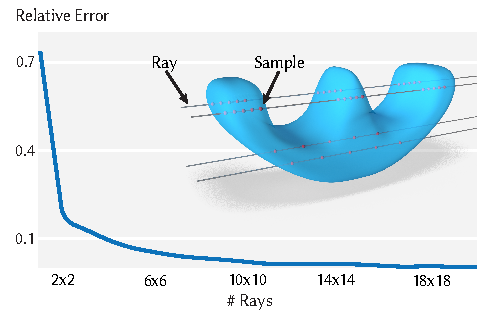
\includegraphics[width=\linewidth]{figures/raycasting_quadrature}
%  \caption{An example raycasting quadrature on a 2D NURBS curve.}
%  \Description{Shows a 2D NURBs curve with horizontal rays intersecting the curve. }
%\end{figure}


%
\section{Results and Discussion}

\begin{table*}[h]
  \setlength{\tabcolsep}{3pt}
  \caption{Performance of, and parameters for the Shape Matching Element Method on all examples. All wall-clock timings are reported in seconds, physical parameters are
  reported with appropriate units. $\rho$ is the applied density, \textbf{E} is the  Young's Modulus and \revise{$\nu$} is the Poisson's ratio.
  \textbf{Sample} is the time taken to sample and construct $\samp{\Jnurbs}$ and $\samp{\Pmatx}$, \textbf{Quad} is the time taken to generate quadrature points via raycasting,
  \textbf{Weights} is the time to compute blending weights, \textbf{Build $\Pi$} is the time to build the projection operator, \textbf{Step} is the average time required to step the simulation (not including collision detection)
  \revise{and \textbf{Nnz} is the ratio of nonzeros to the total number of elements in the stiffness matrix. }
  \revise{We use linearly implicit time integration on all examples and thus the number of step per frame is 1 in the simulation.}
  }
  \label{tbl:perf}
  \begin{center}
  \begin{tabular}{l c c c c c c c c c c c}
   \textbf{Example} & $|\vc{q}|$ & \textbf{Material}&  $\rho$(kg/m$^3$) & \textbf{E}(Pa) & \revise{$\nu$} &\textbf{Sample}(s) & \textbf{Quad}(s)& \textbf{Weights}(s) & \textbf{Build $\Pi$}(s) & \textbf{Step}(s) & \revise{\textbf{Nnz}(\%)} \\
   \hline 
   \rowcolor[HTML]{DAE8FC}
   %\textbf{Cantilever (soft)}       & 564 & Jelly & $1 e^3$ & $1e^6$& 0.45 & $2.53 e^{-2}$ & $4.45 e^{-3}$ & $4.78 e^{-1}$ & $1.86 e^{-1}$ & $1.20 e^{0}$ \\
   %\textbf{Cantilever (stiff)}      & 564 & Rubber & $1 e^3$ & $5 e^6$ & 0.45 & $2.48 e^{-2}$ & $6.37 e^{-3}$ & $5.10 e^{-1}$ & $1.68 e^{-1}$ & $1.19 e^{0}$ \\
   \rowcolor[HTML]{DAE8FC} 
   \textbf{Rocket (soft)}           & 648 & Rubber & $1.27 e^3$ & $7 e^6$ & 0.40 & $2.83 e^{-2}$ & $5.62 e^{-3}$ & $5.58 e^{-1}$ & $6.83 e^{-2}$ & $1.26 e^{0}$ & \revise{100} \\
   \textbf{Rocket (stiff)}          & 648 & Steel & $8 e^3$ & $2 e^{11}$ & 0.32 & $2.56 e^{-2}$ & $5.97 e^{-3}$ & $4.59 e^{-1}$ & $3.48 e^{-2}$ & $9.99 e^{-2}$ & \revise{100} \\
   \rowcolor[HTML]{DAE8FC} 
   \textbf{Starship}                & 750 & Steel & $8 e^3$ & $2 e^{11}$ & 0.32 & $6.78 e^{-2}$ & $1.52 e^{-2}$ & $8.50 e^{-1}$ & $9.52 e^{-2}$ & $6.95 e^{-1}$ & \revise{100} \\
   \revise{\textbf{Beam (twist)}}   & \revise{756} & \revise{Rubber} & \revise{$1 e^3$} & \revise{$1 e^6$} & \revise{0.45} & \revise{$1.97 e^{-1}$} & \revise{$2.25 e^{-2}$} & \revise{$1.35 e^{0}$} & \revise{$5.16 e^{-1}$} & \revise{$3.95 e^{0}$} & \revise{46.94} \\
   \rowcolor[HTML]{DAE8FC} 
   \textbf{Lamppost}                & 942 & Rubber & $3 e^3$ & $1 e^6$ & 0.40 & $1.28 e^{-1}$ & $1.27 e^{-2}$ & $1.89 e^{0}$ & $1.07 e^{0}$ & $2.22 e^{0}$ & \revise{56.38} \\
   \textbf{Tire}                    & 1404 & Rubber/Steel & $2 e^3$/$3 e^3$ & $1 e^6$/$7 e^9$ & 0.47/0.35 & $1.74 e^{-1}$ & $1.32 e^{-2}$ & $1.82 e^{0}$ & $6.79 e^{-1}$ & $1.28 e^{1}$ & \revise{92.5} \\
   \rowcolor[HTML]{DAE8FC} 
   \textbf{Chicken}                 & 1773 & Jelly & $1.27 e^3$ & $1 e^4$ & 0.47 & $9.19 e^{-1}$ & $2.31 e^{-2}$ & $3.38 e^{0}$ & $1.91 e^{0}$ & $1.08 e^{1}$ & \revise{100} \\
   \textbf{Coffee mug (soft)}       & 1800 & Jelly & $1 e^3$ & $1 e^4$ & 0.47 & $4.18 e^{-1}$ & $2.87 e^{-2}$ & $3.77 e^{0}$ & $2.08 e^{0}$ & $1.19 e^{1}$ & \revise{100} \\ 
   \rowcolor[HTML]{DAE8FC} 
   \textbf{Coffee mug (stiff)}      & 1800 & Rubber & $1 e^3$ & $4 e^7$ & 0.40 & $4.15 e^{-2}$ & $1.17 e^{-2}$ & $6.86 e^{-1}$ & $1.09 e^{-1}$ & $5.00 e^{-1}$  & \revise{81.42} \\ 
   \textbf{Castle}                  & 1872 & Jelly & $1.27 e^3$ & $2 e^3$ & 0.45 & $4.84 e^{-1}$ & $1.44 e^{-2}$ & $1.52 e^{0}$ & $5.78 e^{-1}$ & $8.02 e^{0}$ & \revise{100} \\
   \rowcolor[HTML]{DAE8FC} 
   \textbf{Grumpy}                  & 2010 & Jelly & $1 e^3$ & $1 e^4$ & 0.40 & $2.92 e^{-1}$ & $1.23 e^{-2}$ & $2.29 e^{0}$ & $2.89 e^{0}$ & $6.02 e^{0}$ & \revise{84.15} \\    
   \textbf{Astronaut (soft)}        & 3609 & Rubber &  $1.27 e^3$  & $1 e^6$  & 0.47 & $2.47 e^{0}$ & $6.71 e^{-2}$ & $1.13 e^{1}$ & $1.09 e^{1}$ & $1.41 e^{1}$ & \revise{49.04} \\
   \rowcolor[HTML]{DAE8FC} 
   \revise{\textbf{Squid}}          & \revise{4347} & \revise{Jelly} & \revise{ $1 e^3$ } & \revise{$2 e^4$ } & \revise{0.40} & \revise{$4.48 e^{-1}$} & \revise{$2.47 e^{-2}$} & \revise{$1.54 e^{1}$} & \revise{$4.48 e^{1}$} & \revise{$6.73 e^{0}$} & \revise{25.47} \\
   \rowcolor[HTML]{DAE8FC} 
   \hline
  \end{tabular}
  \end{center}
  
  \end{table*}

% \begin{table*}[h]
%   \caption{Performance of, and parameters for the Shape Matching Element Method on all examples. All wall-clock timings are reported in seconds, physical parameters are
%   reported with appropriate units. $\rho$ is the applied density, \textbf{E} is the  Young's Modulus and $\mu$ is the Poisson's ratio.
%   \textbf{Sample} is the time taken to sample and construct $\samp{\Jnurbs}$ and $\samp{\Pmatx}$, \textbf{Quad} is the time taken to generate quadrature points via raycasting,
%   \textbf{Weights} is the time to compute blending weights, \textbf{Build $\Pi$} is the time to build the projection operator and  \textbf{Step} is the average time required to step the simulation (not including collision detection).
%   \revise{We use linearly implicit time integration on all examples and thus the number of step per frame is 1 in the simulation.}
%   }
%   \label{tbl:perf}
%   \begin{center}
%   \begin{tabular}{l c c c c c c c c c c}
%    \textbf{Example} & $|\vc{q}|$ & \textbf{Material}&  $\rho$(kg/m$^3$) & \textbf{E}(Pa) & $\mu$ &\textbf{Sample}(s) & \textbf{Quad}(s)& \textbf{Weights}(s) & \textbf{Build $\Pi$}(s)& \textbf{Step}(s) \\
%    \hline 
%    \rowcolor[HTML]{DAE8FC}
%    %\textbf{Cantilever (soft)}       & 564 & Jelly & $1 e^3$ & $1e^6$& 0.45 & $2.53 e^{-2}$ & $4.45 e^{-3}$ & $4.78 e^{-1}$ & $1.86 e^{-1}$ & $1.20 e^{0}$ \\
%    %\textbf{Cantilever (stiff)}      & 564 & Rubber & $1 e^3$ & $5 e^6$ & 0.45 & $2.48 e^{-2}$ & $6.37 e^{-3}$ & $5.10 e^{-1}$ & $1.68 e^{-1}$ & $1.19 e^{0}$ \\
%    \rowcolor[HTML]{DAE8FC} 
%    \textbf{Rocket (soft)}           & 648 & Rubber & $1.27 e^3$ & $7 e^6$ & 0.40 & $2.83 e^{-2}$ & $5.62 e^{-3}$ & $5.58 e^{-1}$ & $6.83 e^{-2}$ & $1.26 e^{0}$ \\
%    \textbf{Rocket (stiff)}          & 648 & Steel & $8 e^3$ & $2 e^{11}$ & 0.32 & $2.56 e^{-2}$ & $5.97 e^{-3}$ & $4.59 e^{-1}$ & $3.48 e^{-2}$ & $9.99 e^{-2}$ \\
%    \rowcolor[HTML]{DAE8FC} 
%    \textbf{Starship}                & 750 & Steel & $8 e^3$ & $2 e^{11}$ & 0.32 & $6.78 e^{-2}$ & $1.52 e^{-2}$ & $8.50 e^{-1}$ & $9.52 e^{-2}$ & $6.95 e^{-1}$ \\
%    \textbf{Lamppost}                & 942 & Rubber & $3 e^3$ & $1 e^6$ & 0.40 & $1.28 e^{-1}$ & $1.27 e^{-2}$ & $1.89 e^{0}$ & $1.07 e^{0}$ & $2.22 e^{0}$ \\
%    \rowcolor[HTML]{DAE8FC} 
%    \textbf{Tire}                    & 1404 & Rubber/Steel & $2 e^3$/$3 e^3$ & $1 e^6$/$7 e^9$ & 0.47/0.35 & $1.74 e^{-1}$ & $1.32 e^{-2}$ & $1.82 e^{0}$ & $6.79 e^{-1}$ & $1.28 e^{1}$ \\
%    \textbf{Chicken}                 & 1773 & Jelly & $1.27 e^3$ & $1 e^4$ & 0.47 & $9.19 e^{-1}$ & $2.31 e^{-2}$ & $3.38 e^{0}$ & $1.91 e^{0}$ & $1.08 e^{1}$ \\
%    \rowcolor[HTML]{DAE8FC} 
%    \textbf{Coffee mug (soft)}       & 1800 & Jelly & $1 e^3$ & $1 e^4$ & 0.47 & $4.18 e^{-1}$ & $2.87 e^{-2}$ & $3.77 e^{0}$ & $2.08 e^{0}$ & $1.19 e^{1}$  \\ 
%    \textbf{Coffee mug (stiff)}      & 1800 & Rubber & $1 e^3$ & $4 e^7$ & 0.40 & $4.15 e^{-2}$ & $1.17 e^{-2}$ & $6.86 e^{-1}$ & $1.09 e^{-1}$ & $5.00 e^{-1}$  \\ 
%    \rowcolor[HTML]{DAE8FC} 
%    \textbf{Castle}                  & 1872 & Jelly & $1.27 e^3$ & $2 e^3$ & 0.45 & $4.84 e^{-1}$ & $1.44 e^{-2}$ & $1.52 e^{0}$ & $5.78 e^{-1}$ & $8.02 e^{0}$ \\
%    \textbf{Grumpy}                  & 2010 & Jelly & $1 e^3$ & $1 e^4$ & 0.40 & $2.92 e^{-1}$ & $1.23 e^{-2}$ & $2.29 e^{0}$ & $2.89 e^{0}$ & $6.02 e^{0}$  \\    
%    \rowcolor[HTML]{DAE8FC} 
%    \textbf{Astronaut (soft)}        & 3609 & Rubber &  $1.27 e^3$  & $1 e^6$  & 0.47 & $2.47 e^{0}$ & $6.71 e^{-2}$ & $1.13 e^{1}$ & $1.09 e^{1}$ & $1.41 e^{1}$ \\
%    \textbf{Squid}                   & 4347 & Rubber &  $1 e^3$  & $2 e^4$  & 0.40 & $4.48 e^{-1}$ & $2.47 e^{-2}$ & $1.54 e^{1}$ & $4.48 e^{1}$ & $6.73 e^{0}$ \\
%    \rowcolor[HTML]{DAE8FC} 
%    \hline
%   \end{tabular}
%   \end{center}
  
%   \end{table*}

%\dave{we should show the nurbs model in rhino/fusion for every example, maybe an exploded view as well}

%\dave{mention that not so many standard NURBS models so we modelled lots of these ourselves .. show's power of approach that we can model and sim all these examples.}

%\dave{use as many different meshes as possible for figures (i.e try not to have the same mesh show up in more than one figure if possible).}

%\dave{we should report which models we made ourselves}
We implemented SEM using a combination of MATLAB and C++ using both GPToolbox~\cite{gptoolbox} and Bartels~\cite{bartels} for geometry processing and constitutive models 
respectively. Benchmarks were performed using a MacBook Pro with an Intel i5 2.3GHz processor, 16GB of RAM and an Intel Iris Plus Graphics 655 GPU.

\reftbl{perf} shows the size of all our examples along with performance statistics and relevant parameters. 
\revise{We also plot the sparsity patterns of several stiffness matrices in our examples in \reffig{stiffness_sparsity}. }
Note that the individual parts of all models are \emph{not connected}, and no continuity constraints or constructive solid geometry operations have been applied. 
Rather, the SEM approach implicitly couples the boundary parts together to allow for seamless volumetric simulation. 
We use quadratic deformation for all the animation results, except the rocket (stiff) and starship which use linear deformation.
Models were created using Autodesk Fusion 360 \cite{AutodeskFusion360} and \revise{Rhinoceros} 3D 7 \cite{mcneel-rhinoceros}. 
Please see the supplemental video for more animation results.
  
For raycasting operations and rendering we rely on Embree~\cite{10.1145/2601097.2601199} and Blender~\cite{blender}, and triangulate the NURBS surfaces, which only represents an implementation simplification. 
Our core algorithm is not dependent on triangulating the boundary, and an ideal alternative would be using a path tracer that directly accepts NURBS geometry.
For collision detection and handling, for simplicity we use the triangulation to detect inter-penetrations at each iteration, and attempt to move the collided vertex out of its collision surface using a spring-like penalty force, similar to \cite{10.1145/3355089.3356486, 10.1145/2010324.1964932}.
An ideal alternative would be adopting the implicit representation of the surfaces for collision detection and resolution \cite{10.1145/1516522.1516523, 10.1145/3306346.3323010}. 

\nicetohave{Would be nice to mention TNURBS, which would give us a good reason to include the wrench (which i really wanna do). I doubt we have time to do a 3 point bending test, but a simple elastic wrench simulation would be easy to cook up}
For handling trimmed NURBS surfaces, we augment our sampling of the surfaces by using raycasting integration in 2D. Trimmed NURBS may be defined by a boundary curve in the parametric space, so we raycast to find intersection intervals in the UV space on which quadrature points are generated. For rendering Trimmed NURBS, we discretize the the boundary curve as a polyline and use triangle \cite{shewchuk96b, SHEWCHUK200221} to form a boundary conforming triangulation. The vertices of this triangulation serve as fixed set of high resolution UV samples for constructing a render mesh.


%% Results that relate to preprocessing
% weights are good
% \begin{figure}
%   \centering
%   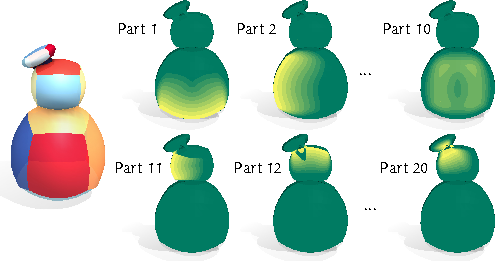
\includegraphics[width=3.33in]{figures/distance_weight_puft.pdf}
%   \caption{Our distance weights decay smoothly from 1.0 (yellow) to 0.0 (green) when moving away from its closest surface. Here we visualize the distribution of the distance weights (with cutoff distance 5.0) corresponding to each part.   
%   }
%   \label{fig:distance_weight_puft}
%   \vspace{-5pt}
% \end{figure} 
% %
% %
% \begin{figure}
%   \centering
%   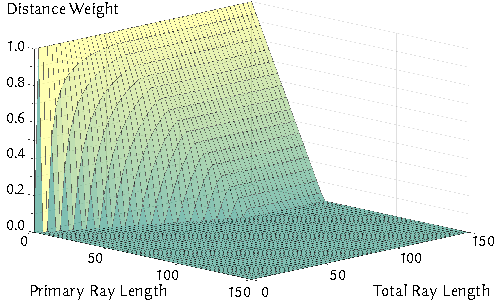
\includegraphics[width=3.33in]{figures/plot_distance_weight.pdf}
%   \caption{We plot the distance weight with respect to the primary and total ray length. Here the cutoff distance is 50.
%   }
%   \label{fig:plot_distance_weight}
%   \vspace{-5pt}
% \end{figure} 

%kinematic model is expressive
% \begin{figure}
%   \includegraphics[width=\columnwidth]{example-image-a}
%   \caption{Take an intesting geometry (maybe that geometry processing cacture), deform it, do our shape matching and then reconstruct the deformed pose. Do this for a bunch of poses (show's kinematic model is good).}
%   \label{fig:deform}
% \end{figure}

%% Results that relate to simulation output
%correctness
\begin{figure}[h]
  \includegraphics[width=\columnwidth]{figures/patch_test.pdf}
  \caption{2D patch test. By applying affine transformations to the boundary of the original undeformed model (left), we show that solving the static problem gives rigid motion for rotation and constant strain for shearing and stretching (right).}
  % \caption{2D patch test. Left: the original undeformed model defined by four surface elements on the boundary. Right:  applying affine transformations to the boundary and show that solving the static problem gives rigid motion for rotation and constant strain for shearing and stretching}
  \label{fig:patchtest}
\end{figure}

\begin{figure}[h]
  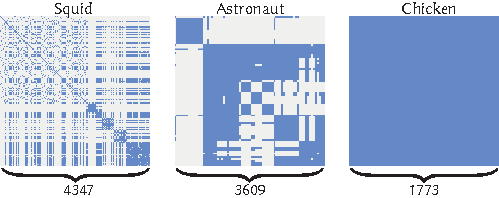
\includegraphics[width=\columnwidth]{figures/stiffness_sparsity.pdf}
  \caption{\revise{Our stiffness matrices can be sparse, while the corresponding matrix has to be dense in the traditional Boundary Element Method \cite{ArtDefo1999}. 
  Sparsity of our stiffness matrix is primarily determined by weight sparsity (number of non-zero weights at a given quadrature point) and polynomial order. }}
  \label{fig:stiffness_sparsity}
\end{figure}

We first validate the physical plausibility of our method using a small 2D patch test~(\reffig{patchtest}). 
Here the test object is a square made of four edges (not joined at the corners) simulated using linear polynomials with a single deformation center.
We apply a battery of boundary conditions and resolve the deformation of the element by minimizing the elastic potential.
We note that SEM is able to represent rigid motions, as well as shearing and anisotropic stretching. 
This implies that, with sparse weights, SEM can resolve these motions locally, leading to physically plausible simulation results.


We demonstrate \emph{qualitative} convergence of SEM with respect to linear tetrahedral finite elements when increasing the number of patches in use.
In \reffig{convergence}, we compare the static configurations of identical cantilevered beams, simulated using a Neohookean constitutive model (Young's Modulus $=$ $0.001$ GPa, Poisson's Ratio $=$ $0.45$). 
\revise{We further perform a basic \emph{quantitative} comparison against FEM by measuring the deflection of the beam at its resting position as we increase the number of patches along the beam. In \reffig{plot_beam_deflection}, the deflection of the SEM beams is reported as a percentage of the FEM beam's deflection.} 

%\begin{wrapfigure}{l}{0.5\columnwidth}
%    	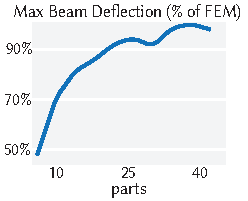
\includegraphics{figures/deflection.pdf}
%	\caption{\revise{Te maximum beam deflection, as a percentage of the FEM beam's maximum deflection, is shown to converge to the FEM result as we add more parts along the beam.}}
%	  \label{fig:plot_beam_deflection}
%\end{wrapfigure}
\begin{figure}[h]
  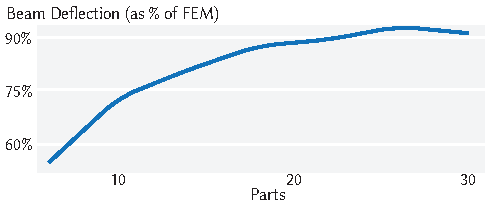
\includegraphics[width=\columnwidth]{figures/deflection_full.pdf}
	\caption{\revise{The SEM beam deflection is plotted as a percentage of the FEM beam's deflection when the beam is at rest. As we subdivide the SEM beam, its deflection converges to the FEM beam's deflection. \ty{currently a very blank figure, which I dont mind, but could consider adding inset beam pictures to give an idea of how this experiment works}}}
  \label{fig:plot_beam_deflection}
\end{figure}

We use SEM with quadratic polynomials for this test and observe that our SEM simulation, made of \revise{26} independent NURBS patches, shows good agreement with FEM. Each subdivision of the NURBS beam enables more complicated kinematics, 
but very few surface elements are needed to produce compelling results.


\begin{figure}[h]
  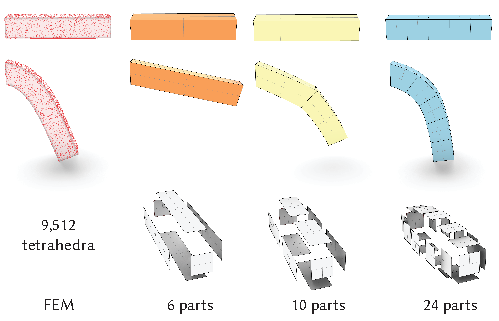
\includegraphics[width=\columnwidth]{figures/beams.pdf}
  \caption{Our SEM simulation is able to qualitatively converge to a high resolution FEM simulation result (left) as we increase the number of surfaces in the model (right). }
  \label{fig:convergence}
\end{figure}

\revise{Additionally, we perform a twisting beam experiment on a 22 part beam model. Despite the relatively small number of NURBS patches, we see in \reffig{beam_twist} that the quadratic polynonmials permit complex deformation.}


\begin{figure}[h]
  \includegraphics[width=\columnwidth]{figures/beam_twist.pdf}
  \caption{\revise{With the left end of the beam held fixed, we show the result of rotating the right end of a 22 part beam up to 360 degrees.}}
  \label{fig:beam_twist}
\end{figure}


\revise{\reffig{scalability} shows a scalability study in which a  unit cube, composed of 6 parts, is extended by appending 4 more parts at a time.
Note that our algorithm scales similarly to standard high-order finite element approaches due to the compact support of our weight functions.}

\begin{figure}[h]
  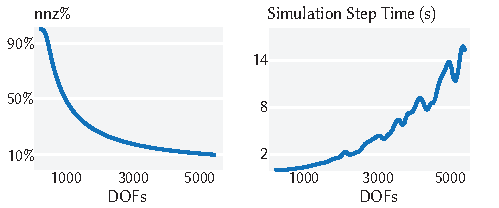
\includegraphics[width=\columnwidth]{figures/scalability.pdf}
  \caption{\revise{Here we progressively add more degrees of freedom to a beam by iteratively inserting 4 part sections, extending the beam in the $x$-axis direction at each step. On the left we report the number of non-zeros as a percentage of the total number of elements in the stiffness matrix (Nnz$\%$). The right plot shows the average runtime of a simulation step as the number of degrees of freedom increases.}}
  \label{fig:scalability}
\end{figure}

We also show that our raycasting weight computation is able to create shape-aware output. \reffig{independence} and \reffig{octopus} show that manipulating
parts that are nearby but separated will behave in an appropriately independent fashion. Our grumpy model is capable of extending 
its leg without causing unrealistic deformations in the plant foot, and our octopus model shows independent motion of all eight limbs upon contact with the ground.


\begin{figure}[h]
  \includegraphics[width=\columnwidth]{figures/independent_movement}
  \caption{Our raycasting weight computation produces shape-aware blending weights. Here the locality of our blending weights allows the two legs of the grumpy model to move independently. }
  \label{fig:independence}
\end{figure}

\begin{figure}[h]
  \includegraphics[width=\columnwidth]{figures/octopus.pdf}
  \caption{\revise{We simulate a falling octopus, and observe the 8 limbs moving independently. Self-collision is not accounted for here.}}
  \label{fig:octopus}
\end{figure}

% relaxed modelling constraints
By virtue of its meshless nature, SEM is robust to a wide range of challenging models with large gaps and disconnected primitives.
\reffig{chicken} shows frames from a simulation of a rubber chicken. Note that the chicken model itself features large gaps between the individual NURBS parts. 
Despite the lack of explicit connectivity, the SEM blending weights have the effect of implicitly enforcing connectivity at these seams. 

\begin{figure*}[htp]
  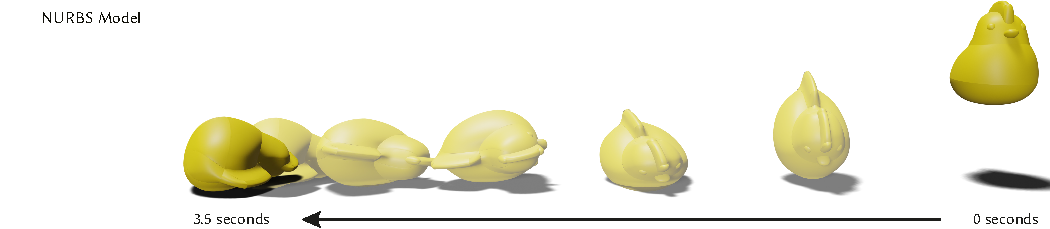
\includegraphics[width=\textwidth]{figures/chicken.pdf}
  \caption{Simulation of a chicken model with gaps between surfaces.}
  \label{fig:chicken}
\end{figure*}

SEM is also robust to intersections in modelling input. \reffig{badmodels} shows simulations of two jelly coffee mugs. 
The top row shows a model with negligible overlap, whereas the bottom row shows the result of a careless modeller who has deeply embedded the handle of the mug in the body in order to attach it, creating a large area of overlap.
In both cases SEM produces a plausible physically-based animation without requiring additional model clean-up.

\begin{figure}[h]
  \includegraphics[width=\columnwidth]{figures/mug_overlap}
  \caption{Our SEM is robust to overlapping regions and self-intersections. Here the simulation result of the coffee mug with overlapping handle (bottom) still matches its corresponding counterpart without negligible overlaps (top). }
  % \caption{Coffee mug with overlapping handle. (top) row of models with increasing overlap (middle) single weight image showing behaviour in the overlapping region, (bottom) simulation result for each one}
  \label{fig:badmodels}
\end{figure}

%different material parameters / material models 
Since the equations of motion for SEM are derived using a general elastic potential, it is theoretically capable of supporting arbitrary elastic constitutive models.
% We derive the equations of motion for SEM using a general elastic potential and thus SEM supports arbitrary constitutive models. 
\reffig{rocket} shows a rocket ship simulated with both high stiffness (steel) and low stiffness materials (rubber). 
In both cases intuitive and visually pleasing results are created wherein the trajectories correctly reflect the desired material characteristics.  
%multiple materials
\begin{figure*}[htp]
  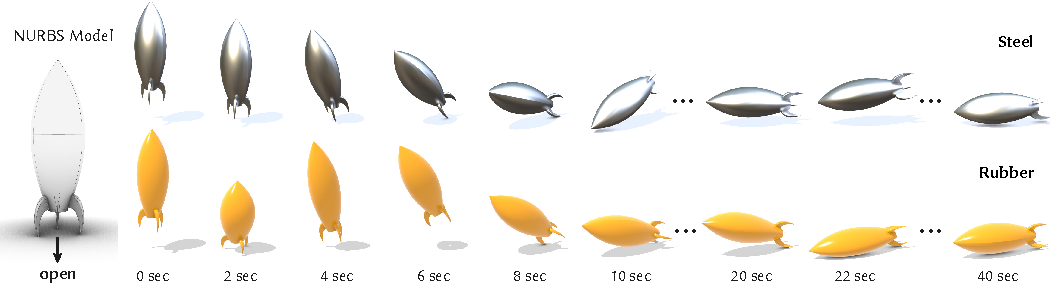
\includegraphics[width=\textwidth]{figures/rocket.pdf}
  \caption{SEM is able to produce animation using a wide variety of material parameters. Here we simulate both a steel and rubber rocket ship. 
  To make this even more challenging, the rocket model is an open surface (at the bottom), but a plausible animation is still generated.}
  \label{fig:rocket}
\end{figure*}

SEM also supports the simulation of objects made up of heterogenous materials. By specifying different material properties inside nested 
parts we are able to simulate a drag racing wheel with a metal hub and soft rubber tread~(\reffig{tire}).

\begin{figure}[h]
  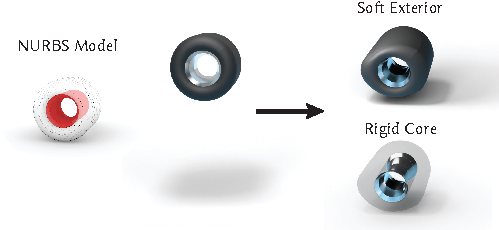
\includegraphics[width=\columnwidth]{figures/tire}
  \caption{Our SEM is directly applicable to the simulation of objects with heterogenous materials.}
  \label{fig:tire}
\end{figure}


% %different surface reps
% Though we focus on NURBS surface representations, the only NURBS specific construction in the SEM method is the Jacobian \refeq{velocity_jacobian}.
% Many other boundary representations admit a linear representation and are thus directly consumable by our method.
% \reffig{subd} shows an example of applying our SEM method to a subdivision model by making such a modification.
% \begin{figure}[h]
%   \includegraphics[width=\columnwidth]{example-image-a}
%   \caption{show subd simulation if we have it. If it works really well we'll just mix subds and nurbs throughout the paper. }
%   \label{fig:subd}
% \end{figure}

% different time integration scheme
\nicetohave{Integration Figure}
%\begin{figure}[h]
%  \includegraphics[width=\columnwidth]{example-image-a}
%  \caption{show mug simulation using newton's method, linearly implicit Euler \Honglin{Maybe I can do that quickly}. }
%  \label{fig:time_integration}
%\end{figure}

%editing example
For downstream applications, the output of  SEM simulation is itself editable in a NURBS modelling program (see \reffig{edit}). 
This can be useful for visual effects pipelines, allowing artists to easily post process animations using the same tools in which they were created.
\begin{figure}[h]
  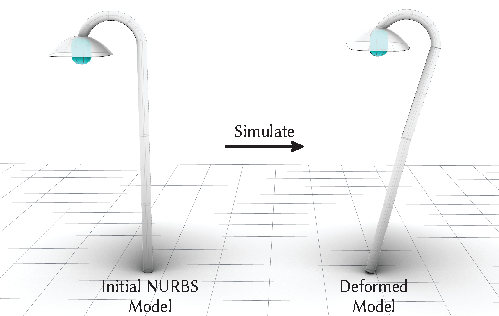
\includegraphics[width=\columnwidth]{figures/export_iges.pdf}
  \caption{Here we show the output of an SEM animation loaded into Rhinoceros 3D 7 for additional editing.\ty{note: initial version of figure. Currently remaking it :)}}
  \label{fig:edit}
\end{figure}

%show stoppers
Finally we show a few additional examples, highlighting the ability of SEM to handle complex simulations involving deformation, contact and friction.
In \reffig{staypuft} we show two astronauts in jaunty space suits collide in zero gravity. 
SEM gracefully allows bounded discontinuities in simulation output to allow for rich motion. 
This is similar to Discontinous Galerkin approaches but in SEM this behavior emerges from the kinematic model, rather than from additional flux terms~\cite{kaufmann2009flexible}.
\revise{Our soft enforcement of part connectivity at boundaries is a result of the weighting function attributing equal weight values to equidistant parts. This equal weighting induces elastic forces that attempt to enforce continuity. In our examples, these discontinuities only introduce minor artifacts affecting the rendering, but this may be addressed using a separate render mesh or by using a representation with explicit connectivity.}

In \reffig{teaser} we directly simulate the NURBS surface model of a bouncy castle under a periodic wind force. 
In \reffig{starship} we show an animation of the Space-V starship landing on Mars in a graceful way. 
This example shows the benefit of NURBS modeling, a relatively small number of primitives can represent a complex shape.
SEM successfully handles the stiff materials, complicated geometry and non-trivial collisions in this scene.

\begin{figure*}[htp]
  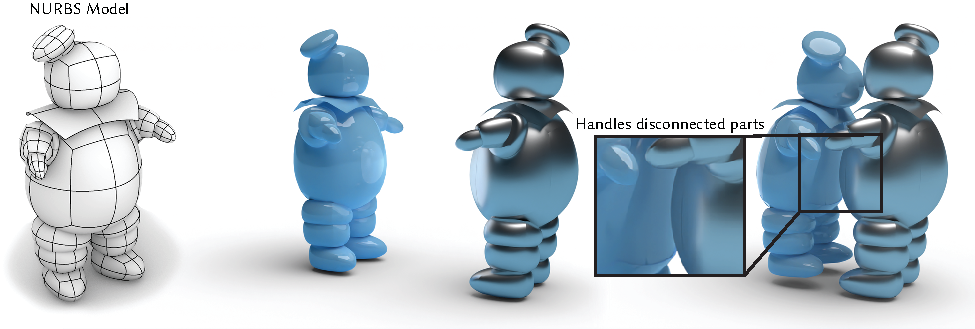
\includegraphics[width=\textwidth]{figures/astronauts.pdf}
  \caption{Two astronauts, in jaunty spacesuits collide while spacewalking in zero-g. SEM correctly handles severely disconnected parts by correctly estimating elastic energy even in discontinuous regions.}
  \label{fig:staypuft}
\end{figure*}

\begin{figure*}[htp]
  \includegraphics[width=\textwidth,height=3in]{figures/starship.pdf}
  \caption{Our SEM is robust to stiff materials, complicated geometry and non-trivial collisions. Here we show the Space-V starship makes a graceful landing on the rugged surface of Mars. }
  \label{fig:starship}
\end{figure*}

\section{Future Work and Conclusions}

%%
%% The next two lines define the bibliography style to be used, and
%% the bibliography file.
\bibliographystyle{ACM-Reference-Format}
\bibliography{references}

\end{document}
